\chapter*{Testing iceberg}

\ifnotes

    Learning outcomes:
    
    \begin{itemize}
        \item Explain why the division between scenarios and programmer tests is not directly described by the pyramid
        \item Describe how to decide if an example should be implemented as a business-readable scenario or as a technical, programmer test
        \item Argue that there should be far more programmer tests than business-readable scenarios/acceptance tests
    \end{itemize}

    The horizontal line is called the "readability waterline". 90\% of an iceberg is beneath the surface of the water.
\fi 

\ifcontent 
    The testing pyramid doesn't help us answer the question:
    
    \setlength{\leftskip}{1cm}
    
        \textit{"When should I write my test using \CUKE{} and when using \JAVA{JUnit}\CSHARP{MsTest}\JAVASCRIPT{a unit testing framework (e.g. Mocha)}\RUBY{a unit testing framework (e.g. RSpec or Test::Unit)}?"}
    
    \setlength{\leftskip}{0pt}
    
    We learnt earlier that \CUKE{} is primarily a collaboration tool, not a test automation tool. So, the answer to the question is:
    
    \setlength{\leftskip}{1cm}
    
        \textit{"When writing the test in business language will help communication."}
    
    \setlength{\leftskip}{0pt}
    
    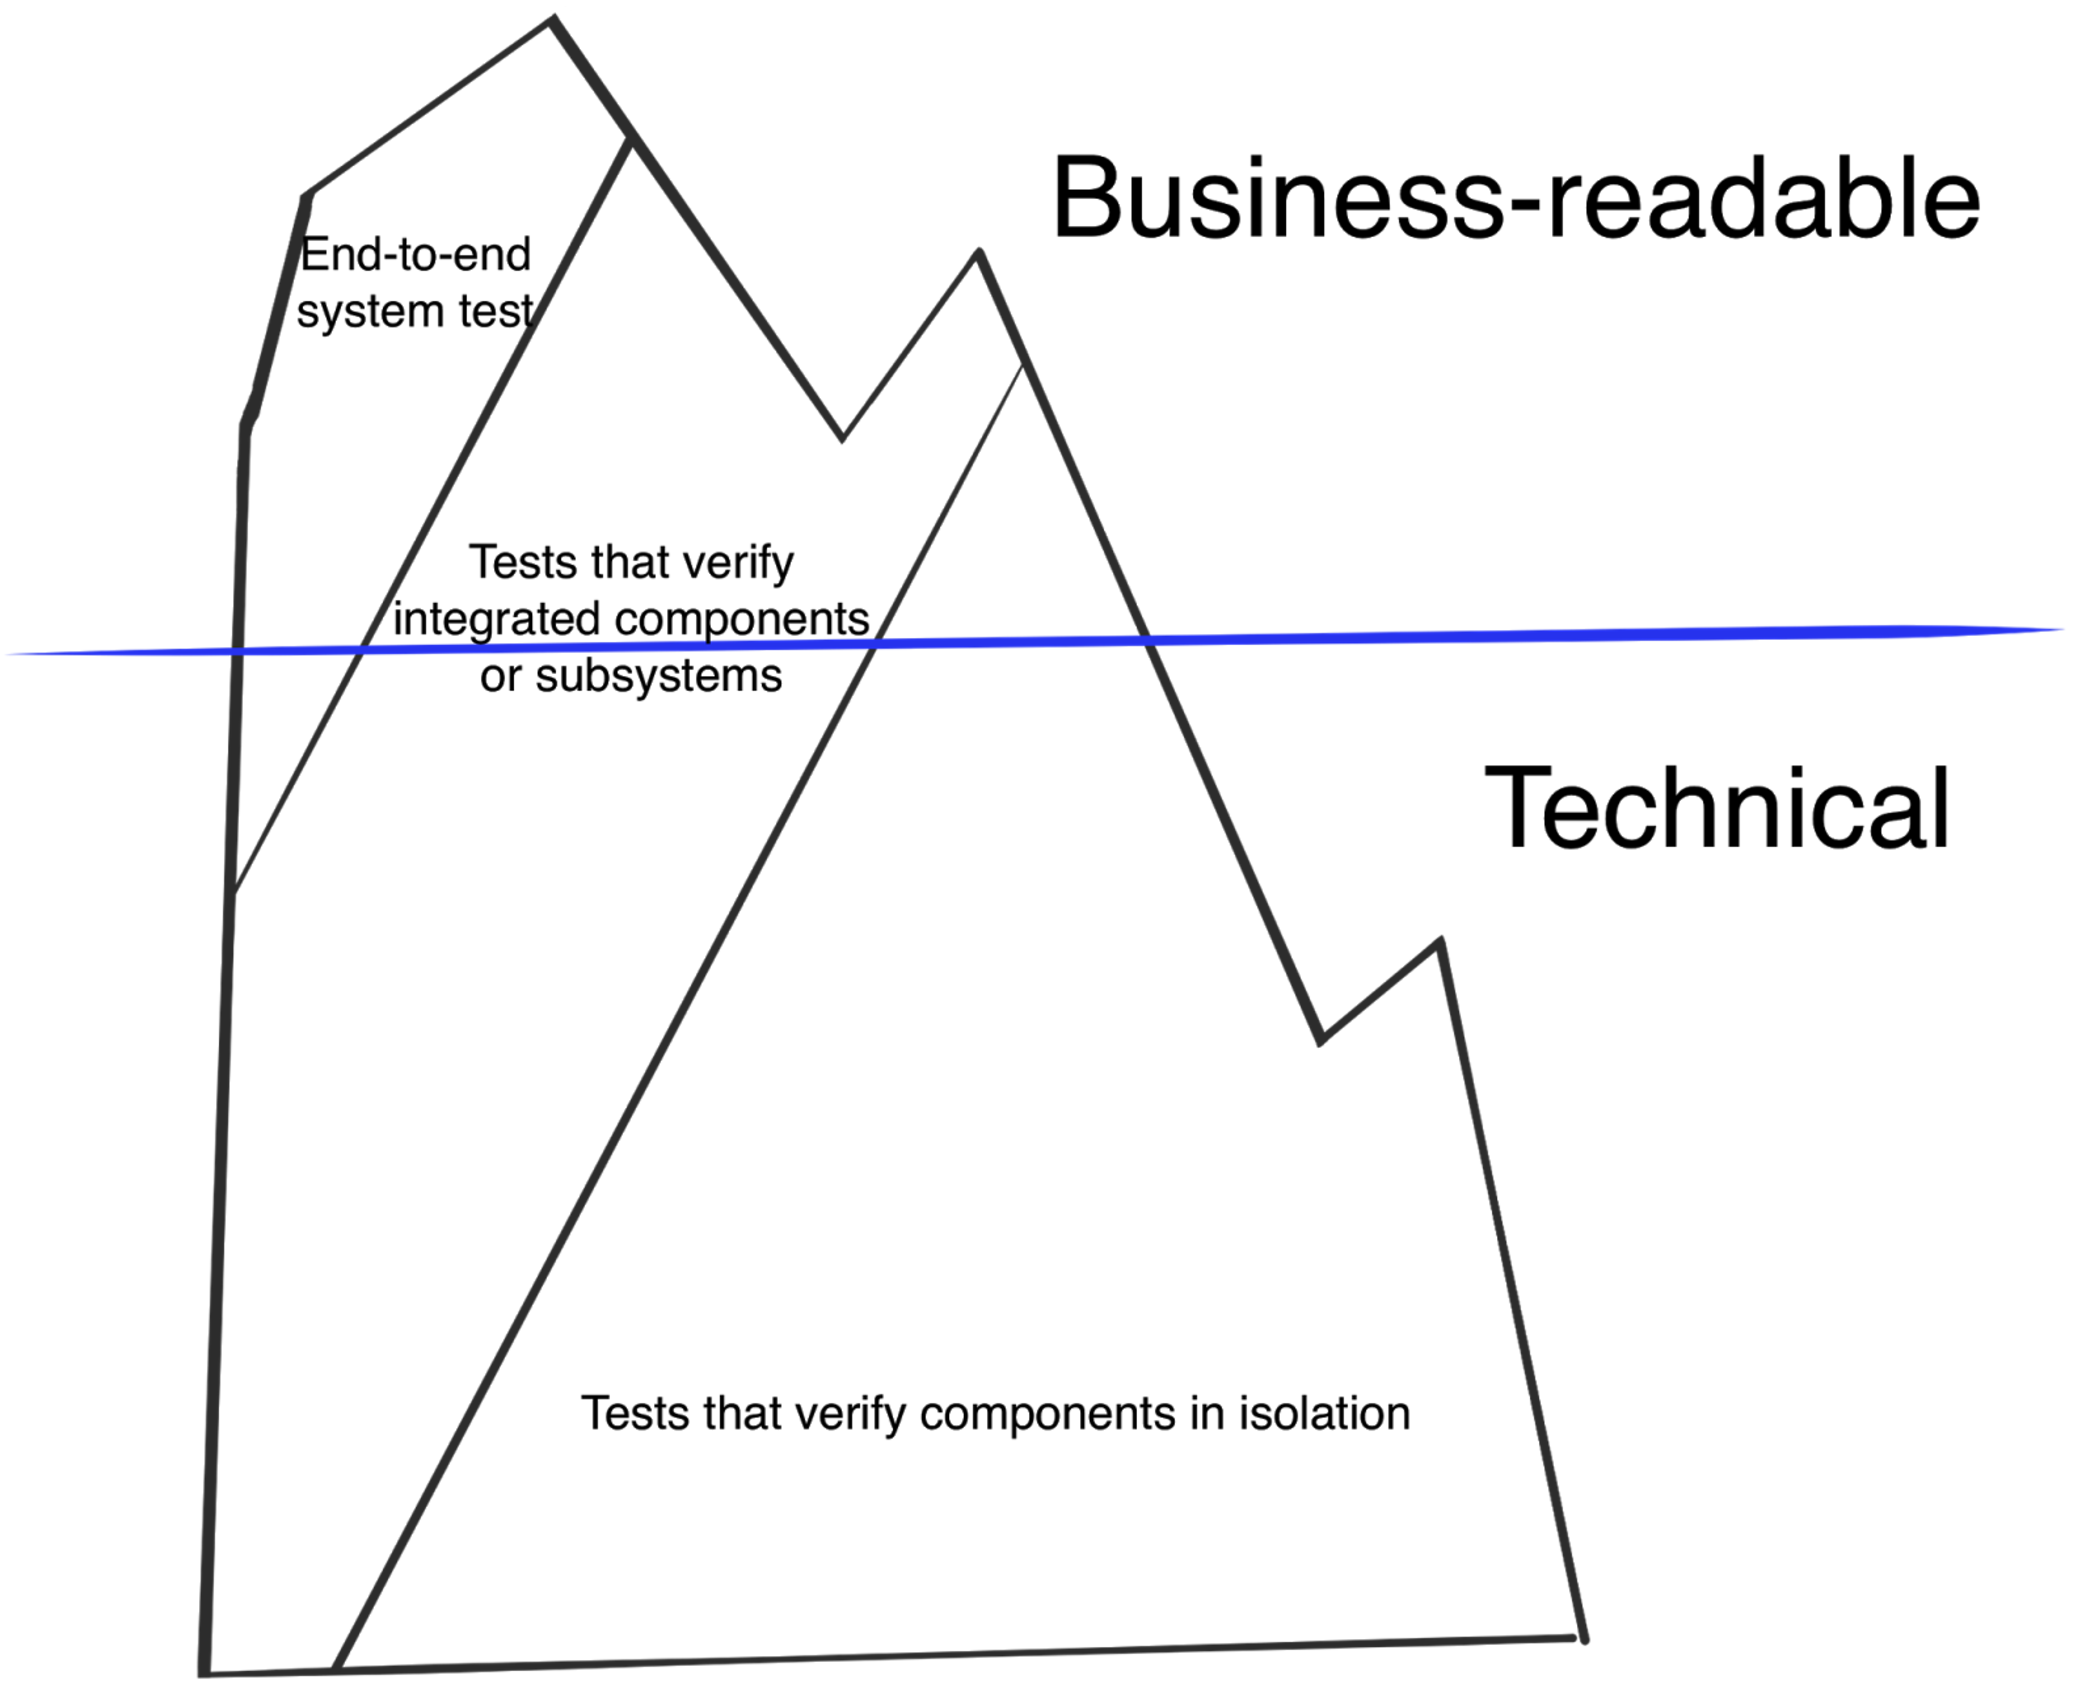
\includegraphics[width=\textwidth]{images/iceberg}
    
    The overriding question when choosing \CUKE{} or your unit testing framework is:
    
    \setlength{\leftskip}{1cm}
    
        \textit{"Will the business be interested enough in this scenario to give meaningful feedback?"}
    
    \setlength{\leftskip}{0pt}
\fi